\documentclass[a4paper,12pt,fleqn]{article}

\usepackage[left=1cm,right=0.5cm,top=0.5cm,bottom=2cm]{geometry}

\usepackage{bfcours}

\def\rdifficulty{1}
\setrdexo{%left skip=1cm,
display exotitle,
exo header = tcolorbox,
%display tags,
skin = bouyachakka,
lower ={box=crep},
display score,
display level,
save lower,
score=\points,
level=\rdifficulty,
overlay={\node[inner sep=0pt,
anchor=west,rotate=90, yshift=0.3cm]%,xshift=-3em], yshift=0.45cm
at (frame.south west) {\thetags[0]} ;}
]%obligatoire
}
\setrdcrep{seyes, correction=true, correction color=monrose, correction font = \large\bfseries}

\newcommand{\tikzinclude}[1]{%
    \stepcounter{tikzfigcounter}%
    \csname tikzfig#1\endcsname
}


\hypersetup{
    pdfauthor={R.Deschamps},
    pdfsubject={},
    pdfkeywords={},
    pdfproducer={LuaLaTeX},
    pdfcreator={Boum Factory}
}
\usepackage{smartdiagram}
%\newcommand{\vocref}[2]{\href{#1}{\color{monrose}#2}}
\usepackage{bfcours-fonts}
\begin{document}

\setcounter{pagecounter}{0}
\setcounter{ExoMA}{0}
\setcounter{prof}{1}

\chapitre[
    \textbf{BF}
    ]{
    Contenu de ce dépot % theme
    }{
    Boum% type_etablissement
    }{
    Factory% nom_etablissement
    }{
    % supplement ( laisser à % si vide )
    }{
    Document explicatif :
    }

    Ce dépot est constitué des outils que j'utilise au quotidien dans mon métier d'enseignant. \\

\setlength{\columnseprule}{0.4pt}
\begin{multicols}{2}
Il pourra intéresser l'\acc{utilisateur débutant} par le \acc{design des environnements} qui ont une \acc{syntaxe simple} d'utilisation. \\
Les \acc{outils numériques} basés sur l'utilisation de bfcours et de \acc{scripts Python fournis} avec ce package facilitent également les \acc{manipulation globales} de code \LaTeX .\\

\columnbreak

Il pourra intéresser l'\acc{utilisateur avancé} par l'intermédiaire des packages de \acc{Régis Deleuze}.\\
Ces derniers sont disponibles dans le \acc{localtexmf/RDProf}. \\
Ils sont très bien documentés (\acc{documentations / rdexo\_doc} ou \acc{documentations / rdcrep\_doc})  et fournissent des \acc{commandes} et \acc{environnements} hautement personnalisables. \\
A mon expérience, je n'ai rien vu d'aussi performant sur les dépots ctan. 

\end{multicols}
Ce package est \acc{compatible} avec les plateformes \acc{MathAlea} et les package \acc{profCollège} et \acc{ProfLycée}.\\

\boite{Pour télécharger le dépot : }{
    \begin{enumerate}
        \item Aller sur \href{https://github.com/Romain1099/BFCours.git}{https://github.com/Romain1099/BFCours.git}
        \item Cliquer sur 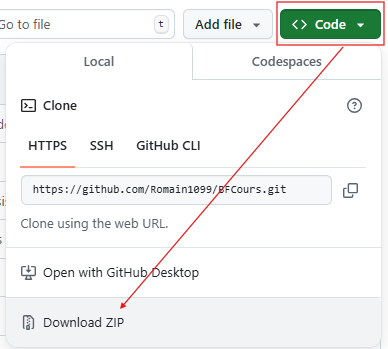
\includegraphics[options]{download_repo.png}
        \item Extraire dans le répertoire de votre choix et \acc{explorer les applications disponibles}.
    \end{enumerate}
}

\begin{center}
    \smartdiagramset{description title width=3cm, 
    description title text width=4.75cm,
    descriptive items y sep=4,
    description text width=5.75cm,
    module minimum height=2.25cm}
    \smartdiagram[descriptive diagram]{%
    {\bfseries \Large \color{blue!75!black} localtexmf/bfcours,\raggedright Le méta-package LaTeX qui contient mes commandes et environnements.\\La documentation pour l'instant 
    très sobre donne une idée des fonctionnalités disponibles. \\
    Des exemples d'utilisations sont disponibles dans le répertoire \frquote{Exemples}.},
    {\bfseries \Large \color{blue!75!black} Assistant\_saisie\_resultats,\raggedright {Module de gestion et d'analyse des résultats avancé}},
    {\bfseries \Large \color{blue!75!black} assistant\_creation\_document,\raggedright Module de gestion de modèles avancé. },
    {\bfseries \Large \color{blue!75!black} Pré-formattage MathAlea, \raggedright Script permettant d'adapter les exercices produits par MathAlea au format optimal pour bfcours. },
    {\bfseries \Large \color{blue!75!black} Tikzdiff,\raggedright Script permettant de stocker le code des figures Tikz dans un document secondaire pour faciliter la saisie d'un document.},
    }
    \end{center}
    

\end{document}